\documentclass[a4]{article}
\pagestyle{myheadings}

%%%%%%%%%%%%%%%%%%%
% Packages/Macros %
%%%%%%%%%%%%%%%%%%%
\usepackage{mathrsfs}


\usepackage{fancyhdr}
\pagestyle{fancy}
\lhead{}
\chead{}
\rhead{}
\lfoot{}
\cfoot{} 
\rfoot{\normalsize\thepage}
\renewcommand{\headrulewidth}{0pt}
\renewcommand{\footrulewidth}{0pt}
\newcommand{\RomanNumeralCaps}[1]
    {\MakeUppercase{\romannumeral #1}}

\usepackage{amssymb,latexsym}  % Standard packages
\usepackage[utf8]{inputenc}
\usepackage[russian]{babel}
\usepackage{MnSymbol}
\usepackage{mathrsfs}
\usepackage{amsmath,amsthm}
\usepackage{indentfirst}
\usepackage{graphicx}%,vmargin}
\usepackage{graphicx}
\graphicspath{{pictures/}} 
\usepackage{verbatim}
\usepackage{color}
\usepackage{color,colortbl}
\usepackage[nottoc,numbib]{tocbibind}
\usepackage{float}
\usepackage{multirow}
\usepackage{hhline}

\usepackage{listings}
\definecolor{codegreen}{rgb}{0,0.6,0}
\definecolor{codegray}{rgb}{1,1,1}
\definecolor{codepurple}{rgb}{0.58,0,0.82}
\definecolor{backcolour}{rgb}{0.95,0.95,0.92}
 
\lstdefinestyle{mystyle}{
    backgroundcolor=\color{backcolour},   
    commentstyle=\color{codegreen},
    keywordstyle=\color{magenta},
    numberstyle=\tiny\color{codegray},
    stringstyle=\color{codepurple},
    basicstyle=\footnotesize,
    breakatwhitespace=false,         
    breaklines=true,                 
    captionpos=b,                    
    keepspaces=true,                 
    numbers=left,                    
    numbersep=5pt,                  
    showspaces=false,                
    showstringspaces=false,
    showtabs=false,                  
    tabsize=2
}
 
\lstset{style=mystyle}

\usepackage{url}
\urldef\myurl\url{foo%.com}
\def\UrlBreaks{\do\/\do-}
\usepackage{breakurl}
\Urlmuskip=0mu plus 1mu



\DeclareGraphicsExtensions{.pdf,.png,.jpg}% -- настройка картинок

\usepackage{epigraph} %%% to make inspirational quotes.
\usepackage[all]{xy} %for XyPic'a
\usepackage{color} 
\usepackage{amscd} %для коммутативных диграмм
%\usepackage[colorlinks,urlcolor=red]{hyperref}

%\renewcommand{\baselinestretch}{1.5}
%\sloppy
%\usepackage{listings}
%\lstset{numbers=left}
%\setmarginsrb{2cm}{1.5cm}{1cm}{1.5cm}{0pt}{0mm}{0pt}{13mm}


\newtheorem{Lemma}{Лемма}[section]
\newtheorem{Proposition}{Предложение}[section]
\newtheorem{Theorem}{Теорема}[section]
\newtheorem{Corollary}{Следствие}[section]
\newtheorem{Remark}{Замечание}[section]
\newtheorem{Definition}{Определение}[section]
\newtheorem{Designations}{Обозначение}[section]




%%%%%%%%%%%%%%%%%%%%%%% 
%Подготовка оглавления% 
%%%%%%%%%%%%%%%%%%%%%%% 
\usepackage[titles]{tocloft}
\renewcommand{\cftdotsep}{2} %частота точек
\renewcommand\cftsecleader{\cftdotfill{\cftdotsep}}
\renewcommand{\cfttoctitlefont}{\hspace{0.38\textwidth} \LARGE\bfseries} 
\renewcommand{\cftsecaftersnum}{.}
\renewcommand{\cftsubsecaftersnum}{.}
\renewcommand{\cftbeforetoctitleskip}{-1em} 
\renewcommand{\cftaftertoctitle}{\mbox{}\hfill \\ \mbox{}\hfill{\footnotesize Стр.}\vspace{-0.5em}} 
%\renewcommand{\cftchapfont}{\normalsize\bfseries \MakeUppercase{\chaptername} } 
%\renewcommand{\cftsecfont}{\hspace{1pt}} 
\renewcommand{\cftsubsecfont}{\hspace{1pt}} 
%\renewcommand{\cftbeforechapskip}{1em} 
\renewcommand{\cftparskip}{3mm} %определяет величину отступа в оглавлении
\setcounter{tocdepth}{5} 
\renewcommand{\listoffigures}{\begingroup %добавляем номер в список иллюстраций
\tocsection
\tocfile{\listfigurename}{lof}
\endgroup}
\renewcommand{\listoftables}{\begingroup %добавляем номер в список иллюстраций
\tocsection
\tocfile{\listtablename}{lot}
\endgroup}


%\renewcommand{\thelikesection}{(\roman{likesection})}
%%%%%%%%%%%
% Margins %
%%%%%%%%%%%
\addtolength{\textwidth}{0.7in}
\textheight=630pt
\addtolength{\evensidemargin}{-0.4in}
\addtolength{\oddsidemargin}{-0.4in}
\addtolength{\topmargin}{-0.4in}

%%%%%%%%%%%%%%%%%%%%%%%%%%%%%%%%%%%
%%%%%%Переопределение chapter%%%%%% 
%%%%%%%%%%%%%%%%%%%%%%%%%%%%%%%%%%%
\newcommand{\empline}{\mbox{}\newline} 
\newcommand{\likechapterheading}[1]{ 
\begin{center} 
\textbf{\MakeUppercase{#1}} 
\end{center} 
\empline} 

%%%%%%%Запиливание переопределённого chapter в оглавление%%%%%% 
\makeatletter 
\renewcommand{\@dotsep}{2} 
\newcommand{\l@likechapter}[2]{{\bfseries\@dottedtocline{0}{0pt}{0pt}{#1}{#2}}} 
\makeatother 
\newcommand{\likechapter}[1]{ 
\likechapterheading{#1} 
\addcontentsline{toc}{likechapter}{\MakeUppercase{#1}}} 




\usepackage{xcolor}
\usepackage{hyperref}
\definecolor{linkcolor}{HTML}{000000} % цвет ссылок
\definecolor{urlcolor}{HTML}{AA1622} % цвет гиперссылок
 
\hypersetup{pdfstartview=FitH,  linkcolor=linkcolor,urlcolor=urlcolor, colorlinks=true}

%%%%%%%%%%%%
% Document %
%%%%%%%%%%%%

%%%%%%%%%%%%%%%%%%%%%%%%%%%%%
%%%%%%главы -- section*%%%%%%
%%%%section -- subsection%%%%
%subsection -- subsubsection%
%%%%%%%%%%%%%%%%%%%%%%%%%%%%%
\def \newstr {\medskip \par \noindent} 



\begin{document}
\newcolumntype{g}{>{\columncolor{codegray}}c}



\def\contentsname{\LARGE{Содержание}}
\thispagestyle{empty}
\begin{center} 
\vspace{2cm} 
{\Large \sc Санкт-Петербургский Политехнический}\\
\vspace{2mm}
{\Large \sc Университет} им. {\Large\sc Петра Великого}\\
\vspace{1cm}
{\large \sc Институт прикладной математики и механики\\ 
\vspace{0.5mm}
\textsc{}}\\ 
\vspace{0.5mm}
{\large\sc Кафедра прикладной математики}\\
\vspace{15mm}
%\rule[0.5ex]{\linewidth}{2pt}\vspace*{-\baselineskip}\vspace*{3.2pt} 
%\rule[0.5ex]{\linewidth}{1pt}\\[\baselineskip] 
{\huge \sc Лабораторная работа №$5$\\
\vspace{6mm}
 }
\vspace*{2mm}
%\rule[0.7ex]{\linewidth}{1pt}\vspace*{-\baselineskip}\vspace{3.2pt} 
%\rule[0.5ex]{\linewidth}{2pt}\\ 
\vspace{1cm}

{\sc $3$ курс$,$ группа $33631/2$}

\vspace{2cm} 
Студент \hfill Д. А. Плаксин\\
\vspace{1cm}
Преподаватель \hfill Баженов А. Н.\\
\vspace{20mm} 

\end{center} 
%\author{Я}
\begin{center}
\vfill {\large\textsc{Санкт-Петербург}}\\ 
2019 г.
\end{center}

%%%%%%%%%%%%%%%%%%%%%%%%%%%%%%%%%%%%%%%%%%%%%%%%%%%%%%%%%%%%%%%%%%%%%%%%%%%%%%%%%%%%%%%%%%%%%%
%\ \\[4cm]

%\rm
%%%%%%%%%%%%%%%%%%%%%%%%%%%%%%%%%%%%%%%%%%%%%%%%%%%%%%%%%%%%%%%%%%%%%%%%%%%%%%%%%%%%%%%%%%%%%%
\newpage
\pagestyle{plain}

%\begin{center}
%\begin{abstract} 

%\end{abstract}

%\end{center}

\newpage
\tableofcontents{}
\newpage
\listoffigures{}
\listoftables{}
\newpage

\section{Постановка задачи}

Необходимо построить выборки объёмом $20, 60, 100, 1000$ для двумерного нормального распределения с коэффициентами корреляции $\rho = 0, 0.5, 0.9$

Вычислить коэффициент корреляции Пирсона, Спирмана и квадрантный коэффициент корреляции для каждой выборки. Эти же вычисления повторить для смеси двумерных нормальных распределений \cite{mix}: 
\begin{equation}
    f(x,y) = 0.9N(x,y,0,0,1,1,0.9)+0.1N(x,y,0,0,10,10,-0.9)
\end{equation}
На графике изобразить точки выборки и эллипс равновероятности.


\section{Теория}

\begin{enumerate}
    \item Двумерное нормально распределение \cite{5_1}:
        \begin{equation}
        N(x,y,0,0,1,1,\rho) = \frac{1}{2\pi\sqrt{1-\rho^2}}e^{-\frac{1}{2(1-\rho^2)}(x^2-2\rho x y+y^2)} \label{dnd}
        \end{equation}
    
    \item Коэффициент корреляции Пирсона \cite{5_2}:
        \begin{equation}
        r_{xy} = \left(\sum\limits_{i=1}^n(x_i-\overline{x})(y_i-\overline{y})\right)\left(\sum\limits_{i=1}^n(x_i-\overline{x})^2\sum\limits_{i=1}^n(y_i-\overline{y})^2\right)^{-\frac{1}{2}} \label{ccp}
        \end{equation}
    \item Коэффициент корреляции Спирмана \cite{5_3}:
        \begin{equation}
        \rho_n = 1 -  \frac{6}{n^3-n}\sum\limits_{i=1}^n d_i^2\label{ccs}
        \end{equation}
        
    \item Квадрантный коэффициент корреляции \cite{5_4}:
        \begin{equation}
        \overset{\wedge}{q} = \frac{1}{n}\sum\limits_{i=1}^n sign(x_i-med\;x)sign(y_i-med\;y)\label{qcc}
        \end{equation}
\end{enumerate}

\section{Реализация}
Работы была выполнена на языке $Python 3.7.$
Для генерации выборок использовался модуль \cite{numpy}.
Для построения графиков использовалась библиотека matplotlib \cite{plotlib}.
Функции распределения обрабатывались при помощи библиотеки scipy.stats \cite{skp}

\section{Результаты}

%\vspace{-2cm}
\begin{figure}[H]
    \centering
    \caption{Графики двумерного нормального распределения\eqref{dnd} при $p=0.0$ }
    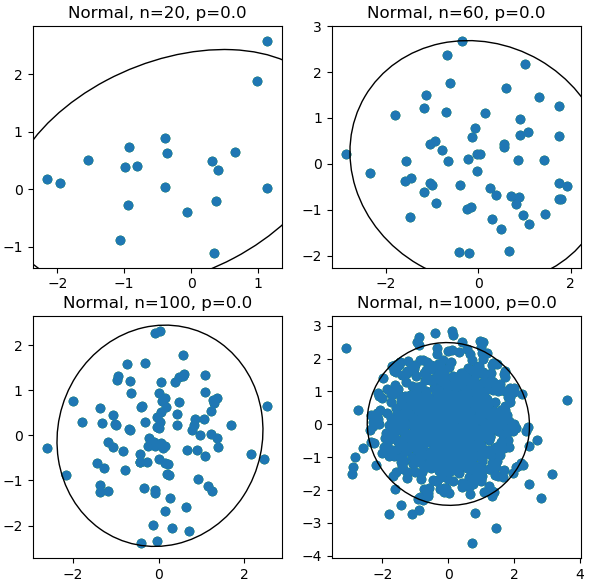
\includegraphics[scale = 0.8]{dotsNormal.png} 
    \label{fig:dis_norm_gis0}
\end{figure}
\begin{table}[H]
\caption{Результаты для двумерного нормального распределения \eqref{dnd} при $p=0.0$}
\label{tab:my_label1}
\begin{center}
\vspace{5mm}
\begin{tabular}{|c|c|c|c|g|c|c|c|c|}
\hhline{----~----}
\multicolumn{4}{|c|}{Normal  $n=20,\;  p=0.0$} &\multirow{11}{*}{$\cdot$} & \multicolumn{4}{c|} {Normal  $n=60,\;  p=0.0$}
\\
\hhline{----~----}
&Pearson     &Spearman    &Quad &   & & Pearson     &Spearman    &Quad        \\    
\hhline{----~----}
		E   &$0.18892$&0.14541&0.06000&  &E   &-0.04642&-0.05109&-0.03333\\
\hhline{----~----}
		$E^2$ &0.05409&0.04186&0.02800&  &$E^2$ &0.01080&0.00965&0.00667\\
\hhline{----~----}
		D   &0.01840&0.02071&0.02440&  &D   &0.00865&0.00704&0.00556\\\rowcolor{codegray}
\hhline{----~----} 
\multicolumn{9}{c}{}\\
\hhline{----~----}
\multicolumn{4}{|c|}{Normal  $n=100,\;  p=0.0$} & & \multicolumn{4}{c|}{Normal  $n=1000,\;  p=0.0$}\\
\hhline{----~----}
&Pearson     &Spearman    &Quad&  & &Pearson     &Spearman    &Quad     \\
\hhline{----~----}
		E   &-0.03469&-0.02805&-0.03200& &E   &0.00805&0.01039&0.00760\\
\hhline{----~----}
		$E^2$ &0.00531&0.00539&0.00864& &$E^2$ &0.00094&0.00083&0.00094\\
\hhline{----~----}
		D   &0.00411&0.00461&0.00762& &D   &0.00088&0.00073&0.00088\\
\hhline{----~----}
\end{tabular}
\end{center}
\end{table}




\vspace{-10cm}
\begin{figure}[H]
    \centering
    \caption{Графики двумерного нормального распределения\eqref{dnd} при $p=0.5$ }
    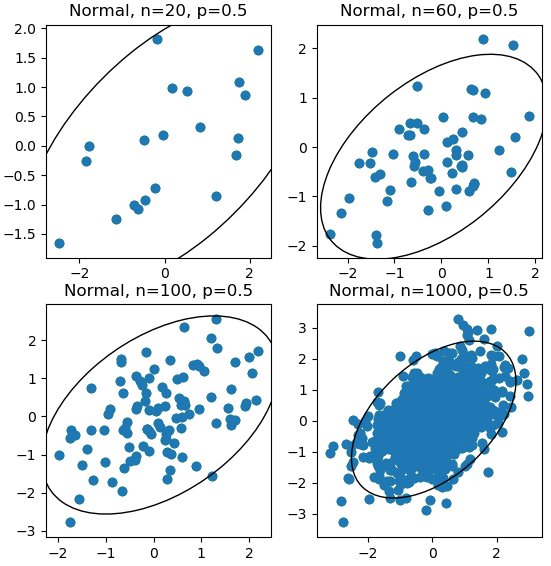
\includegraphics{dotsNormal1.png}
    \label{fig:dis_norm_gis1}
\end{figure}
\begin{table}[H]
\caption{Результаты для двумерного нормального распределения \eqref{dnd} при $p=0.5$}
\label{tab:my_label2}
\begin{center}
\vspace{5mm}
\begin{tabular}{|c|c|c|c|g|c|c|c|c|}
\hhline{----~----}
\multicolumn{4}{|c|}{Normal  $n=20,\;  p=0.5$} &\multirow{11}{*}{$\cdot$} & \multicolumn{4}{c|} {Normal  $n=60,\;  p=0.5$}
\\
\hhline{----~----}
&Pearson     &Spearman    &Quad &   & & Pearson     &Spearman    &Quad        \\    
\hhline{----~----}
		E   &0.50363&0.52647&0.46000&  &E   &0.50847&0.47194&0.31333\\
\hhline{----~----}
		$E^2$ &0.27217&0.30152&0.22800&  &$E^2$ &0.26921&0.23710&0.12222\\
\hhline{----~----}
		D   &0.01853&0.02435&0.01640&  &D   &0.01067&0.01437&0.02404\\\rowcolor{codegray}
\hhline{----~----} 
\multicolumn{9}{c}{}\\
\hhline{----~----}
\multicolumn{4}{|c|}{Normal  $n=100,\;  p=0.5$} & & \multicolumn{4}{c|}{Normal  $n=1000,\;  p=0.5$}\\
\hhline{----~----}
&Pearson     &Spearman    &Quad&  & &Pearson     &Spearman    &Quad     \\
\hhline{----~----}
		E   &0.49628&0.47702&0.33200& &E   &0.49458&0.47938&0.33320\\
\hhline{----~----}
		$E^2$ &0.25200&0.23489&0.12048& &$E^2$ &0.24515&0.23052&0.11207\\
\hhline{----~----}
		D   &0.00570&0.00734&0.01026& &D   &0.00054&0.00071&0.00105\\
\hhline{----~----}
\end{tabular}
\end{center}
\end{table}



\vspace{-1cm}
\begin{figure}[H]
    \centering
    \caption{График двумерного нормального распределения \eqref{dnd} при $p=0.9$ }
    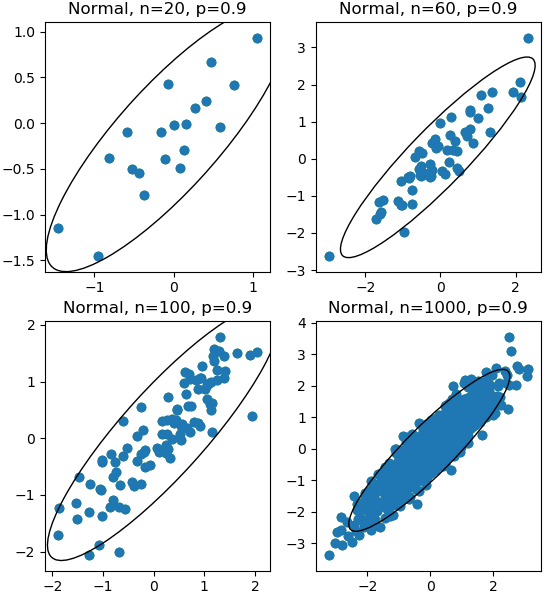
\includegraphics{dotsNormal2.png} 
    \label{fig:dis_norm_gis2}
\end{figure}
\begin{table}[H]
\caption{Результаты для двумерного нормального распределения \eqref{dnd} при $p=0.9$}
\label{tab:my_label3}
\begin{center}
\vspace{5mm}
\begin{tabular}{|c|c|c|c|g|c|c|c|c|}
\hhline{----~----}
\multicolumn{4}{|c|}{Normal  $n=20,\;  p=0.9$} &\multirow{11}{*}{$\cdot$} & \multicolumn{4}{c|} {Normal  $n=60,\;  p=0.9$}
\\
\hhline{----~----}
&Pearson     &Spearman    &Quad &   & & Pearson     &Spearman    &Quad        \\    
\hhline{----~----}
		E   &0.90154&0.85850&0.64000&  &E   &0.89761&0.88464&0.69333\\
\hhline{----~----}
		$E^2$ &0.81558&0.74275&0.44000&  &$E^2$ &0.80681&0.78457&0.48622\\
\hhline{----~----}
		D   &0.00281&0.00574&0.03040&  &D   &0.00112&0.00198&0.00551\\\rowcolor{codegray}
\hhline{----~----} 
\multicolumn{9}{c}{}\\
\hhline{----~----}
\multicolumn{4}{|c|}{Normal  $n=100,\;  p=0.9$} & & \multicolumn{4}{c|}{Normal  $n=1000,\;  p=0.9$}\\
\hhline{----~----}
&Pearson     &Spearman    &Quad&  & &Pearson     &Spearman    &Quad     \\
\hhline{----~----}
		E   &0.89624&0.88888&0.71600& &E   &0.89971&0.88953&0.71120\\
\hhline{----~----}
		$E^2$ &0.80360&0.79094&0.51728& &$E^2$ &0.80951&0.79132&0.50603\\
\hhline{----~----}
		D   &0.00037&0.00082&0.00462& &D   &0.00004&0.00005&0.00022\\
\hhline{----~----}
\end{tabular}
\end{center}
\end{table}





\vspace{-1cm}
\begin{figure}[H]
    \centering
    \caption{Графики смеси двумерных нормальных распределений }
    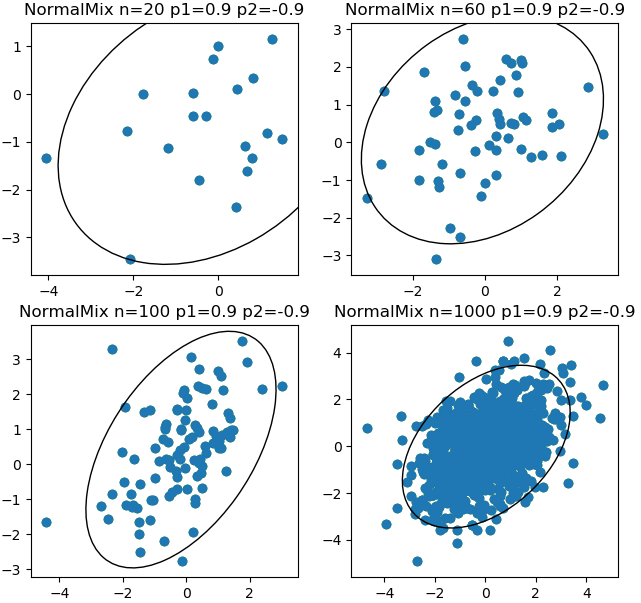
\includegraphics{dotsNormalMix.png} 
    \label{fig:dis_norm_gis4}
\end{figure}
\begin{table}[H]
\caption{Результаты для смеси двумерных нормальных распределений}
\label{tab:my_label4}
\begin{center}
\vspace{5mm}
\begin{tabular}{|c|c|c|c|g|c|c|c|c|}
\hhline{----~----}
\multicolumn{4}{|c|}{NormalMix  $n=20,\;p_1 = 0.9,\;  p_2=-0.9$} &\multirow{11}{*}{$\cdot$} & \multicolumn{4}{c|} {NormalMix  $n=60,\; p_1 = -0.9,\;  p_2=-0.9$}
\\
\hhline{----~----}
&Pearson     &Spearman    &Quad &   & & Pearson     &Spearman    &Quad        \\    
\hhline{----~----}
		E   &0.90154&0.85850&0.64000&  &E   &0.34444&0.33502&0.24000\\
\hhline{----~----}
		$E^2$ &0.12784&0.14056&0.18000&  &$E^2$ &0.13330&0.12744&0.08711\\
\hhline{----~----}
		D   &0.03603&0.04226&0.11240&  &D   &0.01466&0.01521&0.02951\\\rowcolor{codegray}
\hhline{----~----} 
\multicolumn{9}{c}{}\\
\hhline{----~----}
\multicolumn{4}{|c|}{NormalMix  $n=100,\;p_1=0.9,\;  p_2=-0.9$} & & \multicolumn{4}{c|}{NormalMix  $n=1000,\;p_1=0.9,\;  p_2=-0.9$}\\
\hhline{----~----}
&Pearson     &Spearman    &Quad&  & &Pearson     &Spearman    &Quad     \\
\hhline{----~----}
		E   &0.42503&0.39751&0.26400& &E   &0.38948&0.37427&0.25080\\
\hhline{----~----}
		$E^2$ &0.18615&0.16254&0.07584& &$E^2$ &0.15242&0.14103&0.06380\\
\hhline{----~----}
		D   &0.00550&0.00453&0.00614& &D   &0.00073&0.00095&0.00090\\
\hhline{----~----}
\end{tabular}
\end{center}
\end{table}


\section{Выводы}
По таблицам \ref{tab:my_label1}, \ref{tab:my_label2}, \ref{tab:my_label3}, \ref{tab:my_label4}, видно, что, при увеличении объёма выборки, подсчитанные коэффициенты корреляции стремятся к теоретическим.

Ближе всех к данному коэффициенту корреляции находится коэффициент Пирсона.

По графикам видно, что при уменьшении корреляции эллипс равновероятности стремится к окружности, а при увеличении растягивается.



\begin{thebibliography}{}
    \bibitem{numpy}  Модуль numpy  -  https://physics.susu.ru/vorontsov/language/numpy.html
    
    \bibitem{plotlib} 
    Модуль matplotlib - https://matplotlib.org/users/index.html
    
    \bibitem{skp}
    Модуль scipy - https://docs.scipy.org/doc/scipy/reference/
    
\bibitem{mix}
    http://stu.sernam.ru/book\_stat3.php?id=55
    
\bibitem{5_1}
Двумерное нормальное распределение: https://en.wikipedia.org/wiki/Multivariate\_normal\_distribution
\bibitem{5_2}
Коэффициент корреляции Пирса: http://statistica.ru/theory/koeffitsient-korrelyatsii/ 
\bibitem{5_3}
Коэффициент корреляции Спирмана: 
http://economic-definition.com/Exchange\_Terminology/Koefficient\_korrelyacii\_Correlation\_coefficient\_\_eto.html
\bibitem{5_4} Квадрантный коэффициент корреляции: https://www.researchgate.net/profile/Pavel\_Smirnov8/publication/\do-316973167\_Robastnye\_metody\_i\_algoritmy\_ocenivania\_korrelacionnyh\_harakteristik\_dannyh\_na\_os\do-nove\_novyh\_vysokoeffektivnyh\_i\_bystryh\_robastnyh\_ocenok\_masstaba/links/591b019d458515695282\do-8a52/Robastnye-metody-i-algoritmy-ocenivania-korrelacionnyh-harakteristik-dannyh-na-osnove-novyh-vysokoeffektivnyh-i-bystryh-robastnyh-ocenok-masstaba.pdf\#page=81

\end{thebibliography}

\section{Приложения}


Код отчёта:\; \url{https://github.com/MisterProper9000/MatStatLabs/blob/master/MatStatLab5/MatStatLab5.tex}

Код лаборатрной:\; \url{https://github.com/MisterProper9000/MatStatLabs/blob/master/MatStatLab5/MatStatLab5.py}

\lstinputlisting[language=Python]{MatStatLab5.py}

\end{document}
